\chapter{Evaluation}
The objective of this chapter is to review my implementation's success at meeting the original project success criteria. Hence, I start by discussing the project success criteria and how my project device meets them (\S\ref{sec:results}). Then, I assess my implementation according to the following goals:
\begin{itemize}[leftmargin=*, noitemsep]
	\item \textbf{Correctness}: The correctness of the design is assessed using simulation-based verification tests to look for errors (\S\ref{sec:sim}).
	\item \textbf{Functionality}: The functionality of the device is assessed using multiple simulations and hardware-based functional tests (\S\ref{sec:hwtest}).
	\item \textbf{Performance}: The performance of the design is evaluated in various aspects, which are listed in \S\ref{sec:eval}. The analysis also compares the design's performance with that of a standard switch, where appropriate.
\end{itemize}
Finally, I demonstrate the device's interoperability (\S\ref{sec:interop}) and discuss the limitations of the current design (\S\ref{sec:limit}). 

\section{Overall Results}
\label{sec:results}
The success criteria of the project, as described in the original proposal (Appendix \ref{sec:proposal}) and refined in \S\ref{sec:req}, have all been met. They are briefly summarised below, with pointers to the relevant discussion in this document:

\textbf{$\bullet$ Criterion 1}: \textit{Having an implementation of the switch's functionalities in P4 code.}

The P4 code constituted the basis of the project and was completed in the early stage. It was revised many times, based on the code review feedback from my supervisor and the results of simulations and tests. The P4 implementation was described in detail in \S\ref{sec:sw}, while the hardware implementation, which provides the basis to meet Criteria 2 and 3, was discussed in \S\ref{sec:hw}.

\textbf{$\bullet$ Criterion 2}: \textit{The implementation passes two different simulations.}

Simulation and testing is the primary subject of this chapter. The design was simulated through various test cases and passed two different types of simulation: block-level and chip-level simulation. The details are discussed in \S\ref{sec:sim}, including the test data generation process and the test cases chosen.

\textbf{$\bullet$ Criterion 3}: \textit{The implementation works correctly in hardware (functional system test).}

After passing the simulations, the design was compiled and tested on the NetFPGA SUME board. The results are presented in \S\ref{sec:hwtest}.

\textbf{$\bullet$ Criterion 4}: \textit{Able to demonstrate its interoperability with a software-based application.}

Its interoperability was demonstrated in \S\ref{sec:interop} using two simple applications: \verb|ping| and \verb|iperf3|.

\textbf{$\bullet$ Criterion 5}: \textit{Provide a performance evaluation of the design.}

The performance of the design is measured using three metrics: latency, throughput and resources utilisation. It is then analysed in comparison to the performance of a standard switch written in Verilog \cite{refswitch, refswitchbf} and evaluated. The results are presented in \S\ref{sec:eval}.

\textbf{$\bullet$ Extension 1}: \textit{Sending a notification to the source if multiple retransmissions fail.}

With the current system architecture, the switch will retransmit \textit{once} if it receives three DUP ACKs. If the retransmission fails, subsequent DUP ACK packets will be sent back to the sender normally. This was implemented using the \verb|retransmit_cnt_reg_ifElseRaw| extern, which was discussed in \S\ref{sec:extern}.

\textbf{$\bullet$ Extension 2}: \textit{Provide an evaluation in comparison to a standard switch performance.}

A standard switch design \cite{refswitch, refswitchbf} was also tested for performance using the same metrics. The results are used to compare with the project design performance in \S\ref{sec:perf} and \S\ref{sec:limit}, where the difference in the performance is also discussed.

\section{Simulation Environment}
\label{sec:sim}
It is generally easier to debug program behaviour in simulation than in hardware, and the purpose of the simulation environment is exactly that. For this purpose, the P4$\rightarrow$NetFPGA workflow provides a simulation environment with automated test infrastructure. There are two types of simulation: block-level simulation (SDNet simulation) and chip-level simulation (SUME simulation). The SDNet simulation covers the correctness of the P4 implementation on packet-level. It checks that the output port and the correct signal to the cache queue were set correctly in the packet's \verb|sume_metadata| and \verb|digest_data| respectively. The SUME simulation, on the other hand, tests scenarios that cannot be covered by the SDNet simulation. For example, when the third DUP ACK packet is received, the P4 code modifies \verb|digest_data.tuser| to signal the cache queue to retransmit the packet in port \verb|nf1|. In SDNet simulation, we only expect to see one packet coming out of port \verb|nf0| with its \verb|digest_data.tuser| modified. However, in SUME simulation, we expect to observe the retransmitted packet as well. Thus, even if the inputs are the same as the SDNet simulation, the expected outputs and functionalities are different in the SUME simulation.

To run a simulation, we provide the corresponding test bench with the appropriate scripts. We will modify the following example files, which are provided by the P4$\rightarrow$NetFPGA workflow:

For \textbf{SDNet simulation}:
\begin{itemize}[leftmargin=*, noitemsep]
	\item \texttt{commands.txt}: used to generate the control plane functionality. As such, it contains the set of commands to add entries to the match-action tables that we have defined in our P4 program (see Table \ref{tab:forward} and \ref{tab:retransmit}). These entries will be used in the SUME simulation and by the SUME board.
	\item \texttt{gen\_testdata.py} uses \verb|scapy| library to generate test packets (\& metadata), along with the corresponding expected output packets and metadata. P4$\rightarrow$NetFPGA compares the output file with the expected output to give the result. This script also generates \verb|.pcap| files from the test packets that will be used in the SUME simulation.
\end{itemize}
For \textbf{SUME simulation}:
\begin{itemize}[leftmargin=*, noitemsep]
	\item \texttt{nf\_test.py} runs the SUME simulation by executing \texttt{run.py}.
	\item \texttt{run.py} reads the packet traces (\verb|.pcap| files) generated by the \texttt{gen\_testdata.py} script and/or creates new packets and applies them to the SUME interfaces. It also defines a test sequence, including configuration and timing stimulus.
\end{itemize}

\subsection{Test Data Generation}
The \texttt{gen\_testdata.py} template provided by the P4$\rightarrow$NetFPGA workflow has two functions---\verb|applyPkt()| and \verb|expPkt()|---which allow us to specify input packets and expected output packets respectively. I wrote the \verb|digest_data.py| module and used Python \texttt{scapy} module to generate the metadata and test packets. Figure \ref{fig:pkt} shows how to create and send a test packet, and specify the expected packet. We create the packet headers using \texttt{scapy}'s \texttt{Ether}, \texttt{IP} and \texttt{TCP} classes, stacking the layer with the \texttt{/} operator and pad it to 64 bytes with the \texttt{pad\_pkt()} method. Then, \verb|applyPkt()| will ``send'' the packet to the SimpleSumeSwitch module. Now, we need to specify how we would expect the output packet. We create two variables, \verb|flow_id| and \verb|actions|, to represent the values of the flow identifier and the \verb|digest_data.tuser| field of the output packet. Finally, we use \verb|expPkt()| to put the packet into a list of ``expected'' packets.

\begin{figure}[!h]
{\renewcommand{\baselinestretch}{0.8}\small
	\begin{verbatim}
    from scapy.all import *
    import digest_data
	
    MAC_src = "08:11:11:11:11:08" # Source MAC addr.
    MAC_dst = "08:22:22:22:22:08" # Destination MAC addr.
    sport = 55 # Source L4 port 
    dport = 75 # Destination L4 port
    IP_src = "10.0.0.1" # Source IP addr.
    IP_dst = "10.0.0.2" # Dest IP addr.
	
    pkt = (
      Ether(src=MAC_src, dst=MAC_dst)
      / IP(src=IP_src, dst=IP_dst)
      / TCP(sport=sport, dport=dport, flags="S", seq=1)
    )                              # create the packet using scapy Ether, IP 
                                   # and TCP classes.
    pkt = pad_pkt(pkt, 64)         # pad the packet to 64 bytes
    applyPkt(pkt, "nf0", 0)        # send from port 0

    # compute the flow number
    flow_id = digest_data.compute_flow_number(IP1_src, IP1_dst,
                    6, sport, dport)
    
    # write to port 1 of cache_queue
    actions = digest_data.compute_tuser(0, 0, 0, 
                    tuser_map["nf1"])             
    
    # expect from port 1 of output_queue
    expPkt(pkt, "nf1", drop=False, flow_id=flow_id, tuser=actions)
	\end{verbatim}
}
\caption{A Python code snippet to create test packets and specify the expected output.}
\label{fig:pkt}
\end{figure}

To assess the correctness of the P4 implementation, I used the five following tests in sequence:

\textbf{Test \#1}: \textit{Basic packet forwarding of the SimpleSumeSwitch module.}
\begin{enumerate}[label*=\arabic*.,leftmargin=*, noitemsep]
	\item \textbf{Goal}: Test that the program correctly forwards a packet and modifies its metadata.
	\item \textbf{Input}: Send 1 packet from port \verb|nf0| to port \verb|nf1|. This packet belongs to a flow of interest. 
	\item \textbf{Expected output}: Expect 1 packet coming out of port \verb|nf1| with the \verb|digest_data.flow_id| field computed and matches the flow identifier of the input packet, and \verb|digest_data.tuser| set to signal the cache queue to buffer the packet in port \verb|nf1|.
\end{enumerate}

\textbf{Test \#2}: \textit{Program behaviour when standard ACK packets are received.}
\begin{enumerate}[label*=\arabic*.,leftmargin=*, noitemsep]
	\item \textbf{Goal}: Test that the program correctly signals the cache queue to drop buffered packets that have been acknowledged.
	\item \textbf{Input}: Send 3 packets, all of which belong to a flow of interest, from port \verb|nf0| to port \verb|nf1|. Send 1 ACK packet to port \verb|nf0| acknowledging the receipt of the first packet. Send the 2$^{nd}$ ACK packet to acknowledge the receipt of the remaining two packets.
	\item \textbf{Expected output}: Expect 2 ACK packets coming out of port \verb|nf0|. The first packet has \verb|digest_data.tuser| set to drop 1 packet from port \verb|nf1|. The second packet has \verb|digest_data.tuser| set to drop the remaining 2 packets from port \verb|nf1|.
\end{enumerate}

\textbf{Test \#3}: \textit{Program behaviour when three DUP ACK packets are received.}
\begin{enumerate}[label*=\arabic*.,leftmargin=*, noitemsep]
	\item \textbf{Goal}: Test that the program correctly signals the cache queue to \textbf{retransmit} the required packet.
	\item \textbf{Input}: Send 1 packet from port \verb|nf0| to port \verb|nf1|. Send 3 DUP ACK packets from port \verb|nf1| to port \verb|nf0| requiring for the first packet.
	\item \textbf{Expected output}: Expect the third DUP ACK packet coming out of port \verb|nf0| with its ACK flag set to 0, and \verb|digest_data.tuser| set to signal the cache queue to resend the packet in port \verb|nf1|.
\end{enumerate}

\textbf{Test \#4}: \textit{Program behaviour when a fourth DUP ACK packet is received.}
\begin{enumerate}[label*=\arabic*.,leftmargin=*, noitemsep]
	\item \textbf{Goal}: Test that the program correctly sends the subsequent DUP ACK packets back to the sender normally (i.e. only retransmit once).
	\item \textbf{Input}: Send 1 packets, all of which belong to a flow of interest, from port \verb|nf0| to port \verb|nf1|. Send 1 ACK packet acknowledging the first packet. Send the 2$^{nd}$ ACK packet to acknowledge the remaining two packets.
	\item \textbf{Expected output}: Expect the ACK packet coming out of port \verb|nf0| to be sent back to the sender without any modification.
\end{enumerate}

\textbf{Test \#5}: \textit{Program behaviour when there are multiple flows, only one of which is a flow of interest.}
\begin{enumerate}[label*=\arabic*.,leftmargin=*, noitemsep]
	\item \textbf{Goal}: Test that the program correctly monitors the interested flow (of a latency-sensitive application) and delivers packets of other flows normally.
	\item \textbf{Input}: Create 3 flows and randomly interleave their packets. Send them from port \verb|nf0| to \verb|nf1|.
	\item \textbf{Expected output}: Expect to see that the packets from our interested flow are modified accordingly---buffered, dropped or retransmitted---while the other packets are delivered normally.
\end{enumerate}

After creating the packets and specifying the expected outputs, we proceed to simulate our design.

\subsection{SDNet Simulation}
First, we compile our P4 code with the SDNet compiler. After successful compilation, we run the SDNet simulation using Vivado Simulator (\S\ref{sec:p4-netfpga}). The simulator will ``send'' the user-defined input packets and metadata to the SimpleSumeSwitch HDL module and compare the packets at the output of the P4 switch with the expected packets we specified in \verb|gen_testdata.py|.

A total of 29 packets were used in the tests. Figure \ref{fig:sdnetsim} shows all the packets are received and their metadata are modified as we expected. If the simulation output results in a metadata error (i.e. a mismatch between expected and actual tuples), we can debug using a script to parse the metadata into more readable form and check which fields do not match (Figure \ref{fig:sdnet-err}).

\begin{figure}[!h]
	\centering
	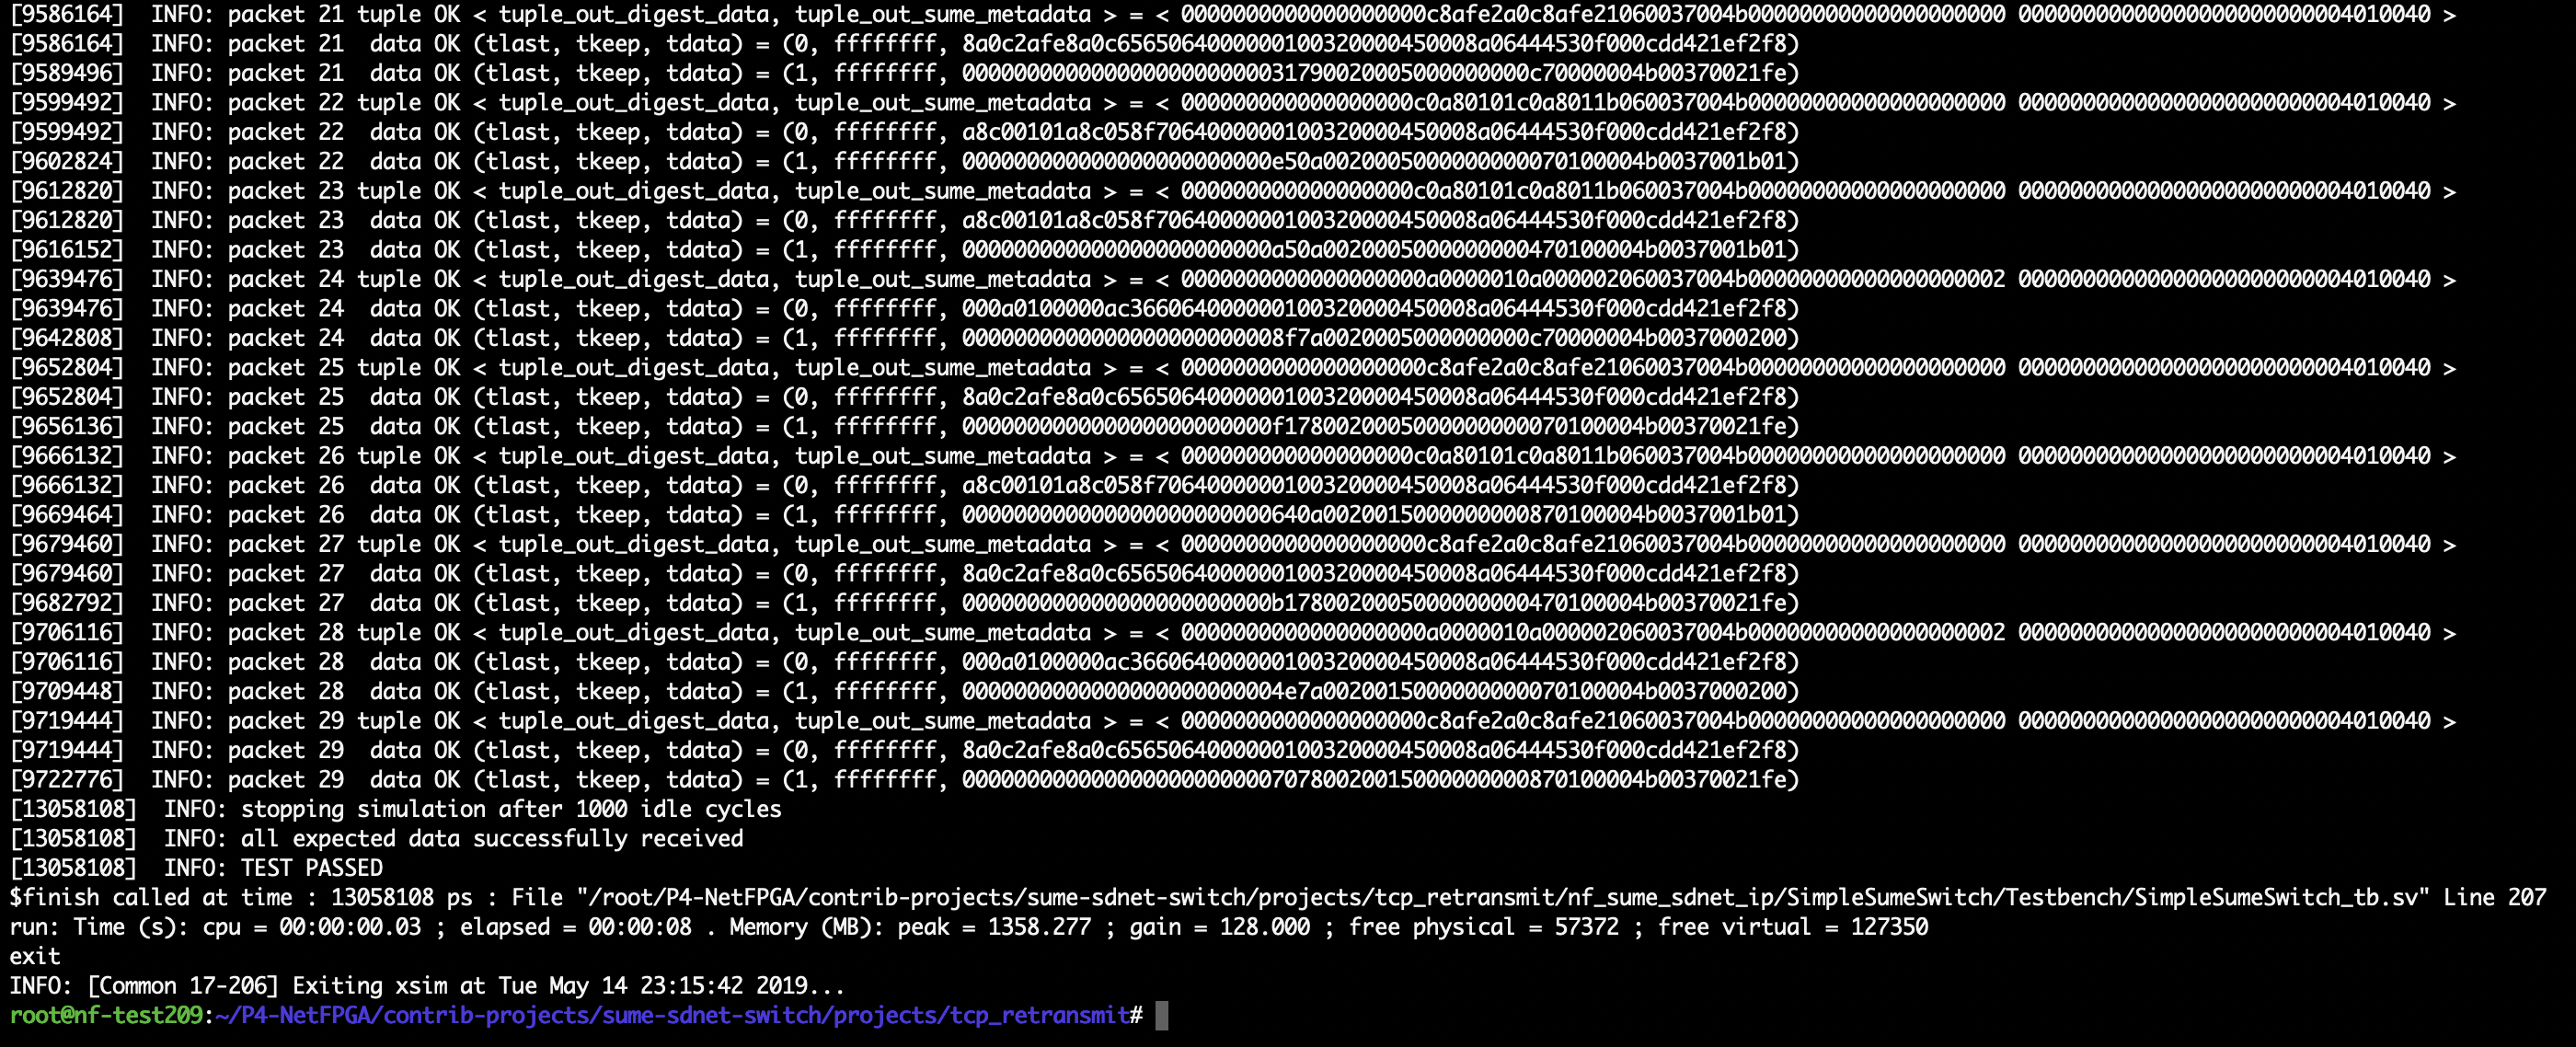
\includegraphics[width=\textwidth]{sdnetsim.png}
	\caption{Test output of the SDNet simulation using Vivado Simulator showing success.}
	\label{fig:sdnetsim}
\end{figure}

\begin{figure}[!h]
	\centering
	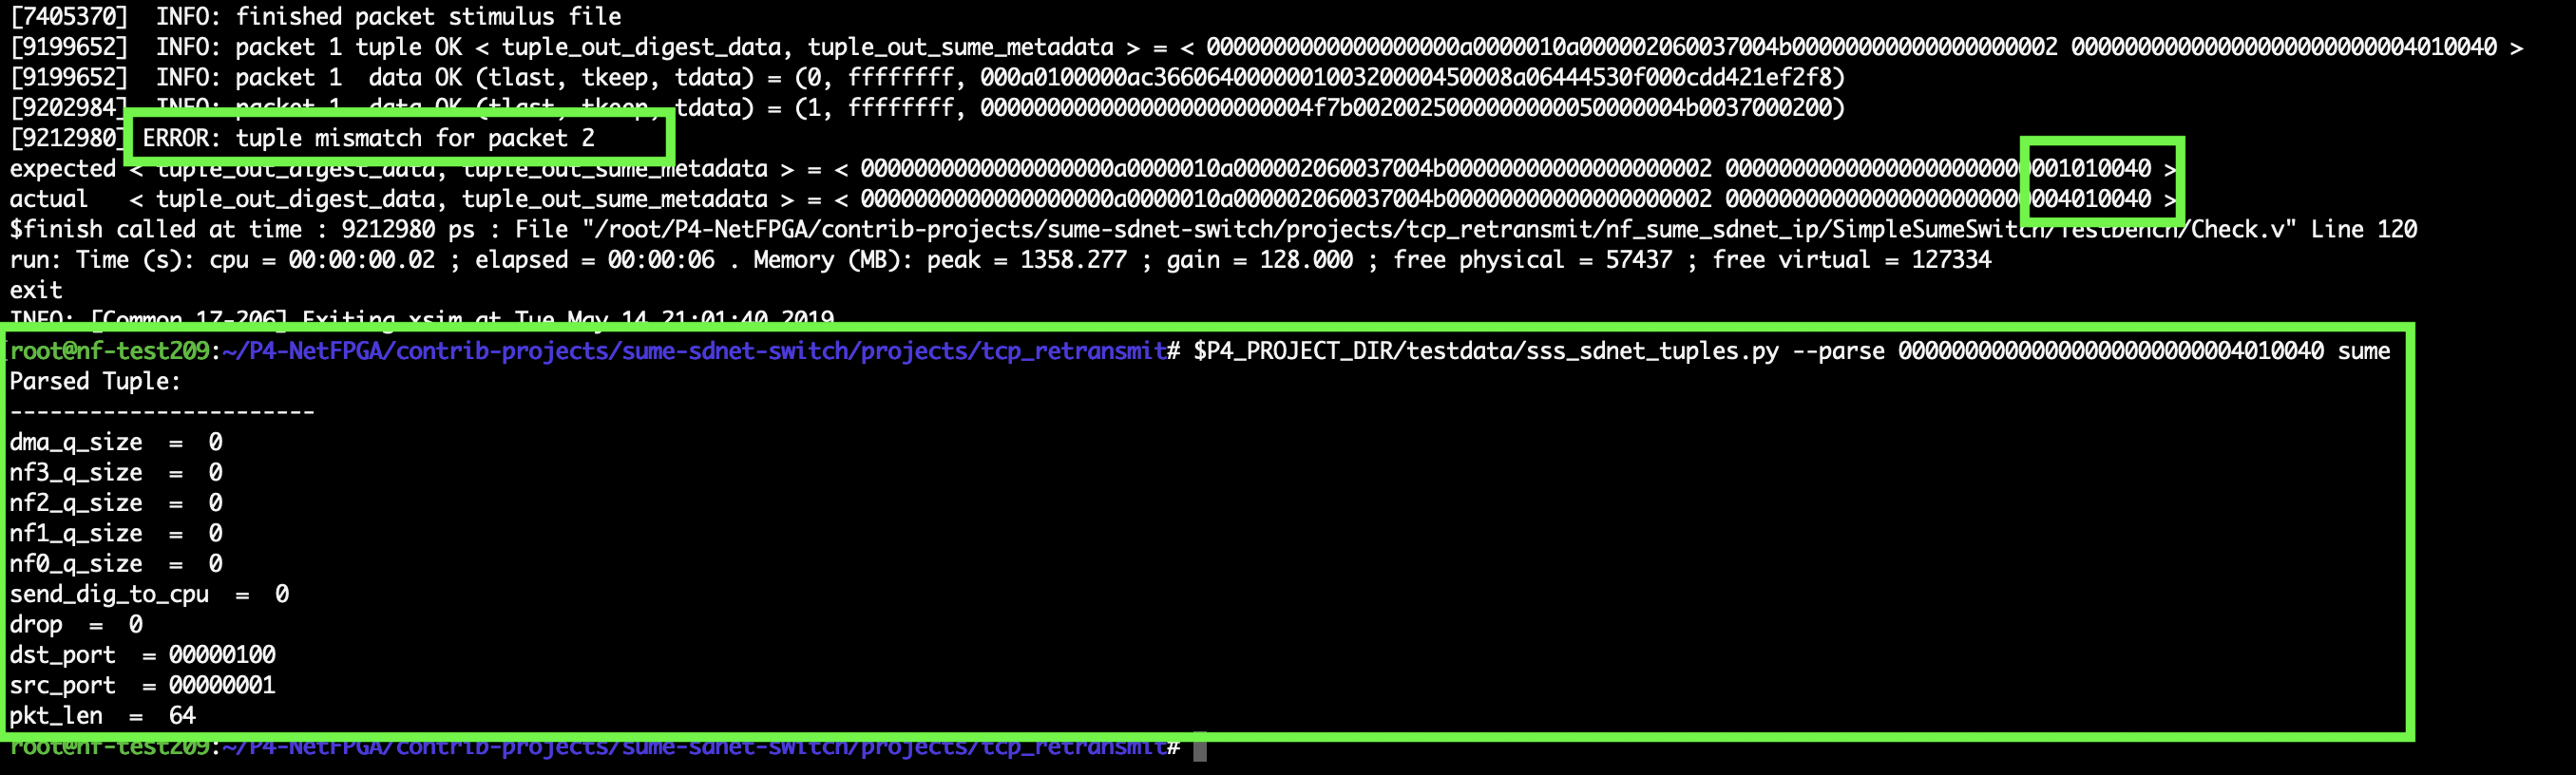
\includegraphics[width=\textwidth]{sdnet-err.png}
	\caption{Test output of SDNet simulation showing error. Using a Python script to parse the metadata into more readable form, we can debug our program.}
	\label{fig:sdnet-err}
\end{figure}

\subsection{SUME simulation}
The SUME simulation installs the SimpleSumeSwitch HDL module as a NetFPGA IP core and simulates the behaviour of the entire NetFPGA reference switch design. This way, it can cover those scenarios that involve the cache queue, which the SDNet simulation cannot. 

I used the same stimuli as the SDNet simulation to verify that the SimpleSumeSwitch module was successfully integrated into our modified reference switch pipeline and assess its correctness. The 
outcome for the tests are mostly the same. The only noticeable difference is in \textbf{Test \#4}, where we received a third DUP ACK packet. We would expect the cache queue to retransmit the packet in port \verb|nf1|, hence an extra packet. Figure \ref{fig:sumelog} shows that we indeed receive the retransmitted packet, which makes the total number of packets 30. Figure \ref{fig:sumesim} illustrates this further by showing the traces of packets leaving port \verb|nf0| and \verb|nf1| of the output queue and the cache queue. There is one packet that coming out of port \verb|nf1| of the cache queue, which is the retransmitted packet.

\begin{figure}[!h]
	\centering
	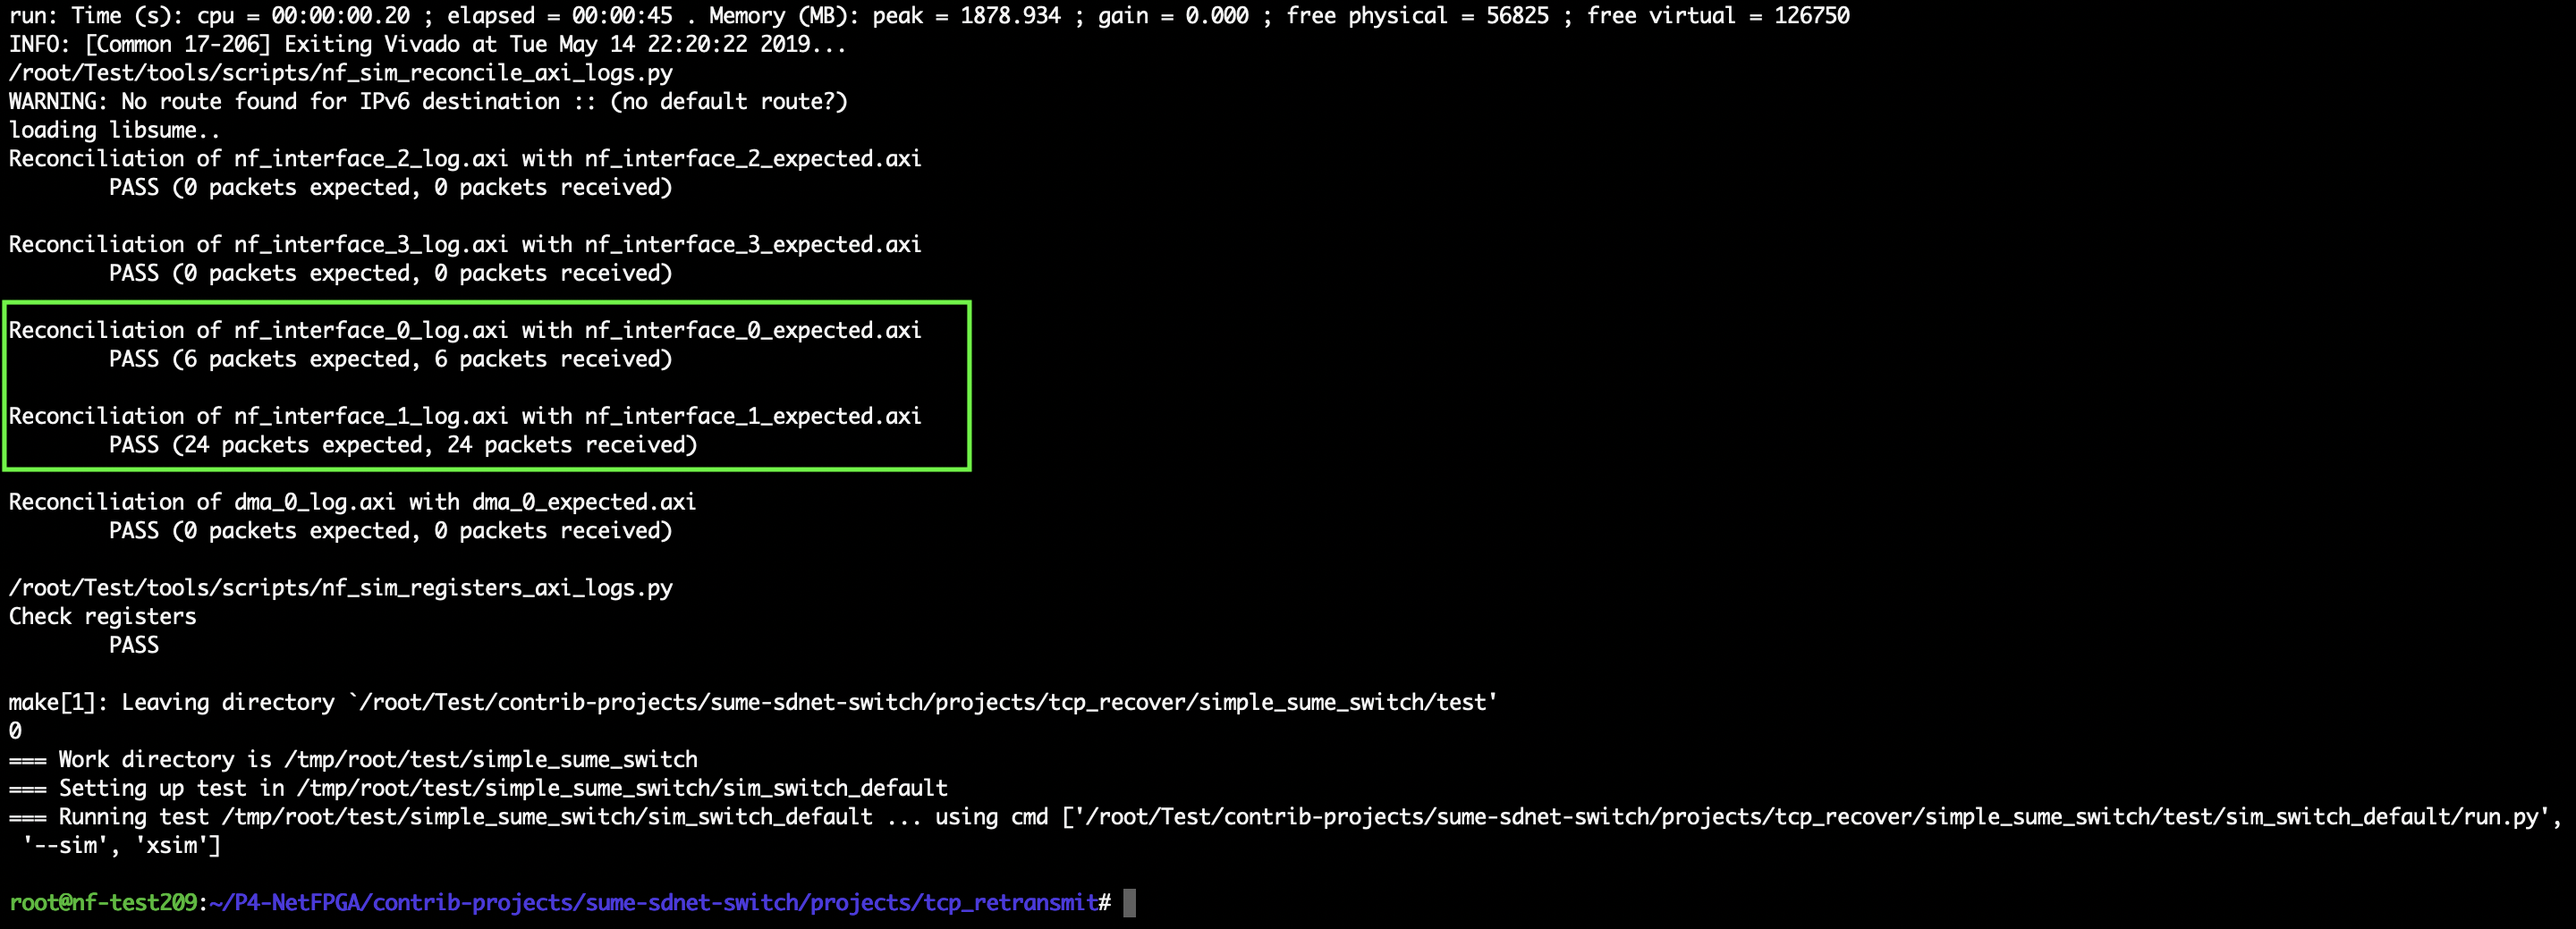
\includegraphics[width=\textwidth]{sume-log.png}
	\caption{Test output of the SUME simulation using Vivado Simulator showing success. We now receive 30 packets instead of 29.}
	\label{fig:sumelog}
\end{figure}

\begin{figure}[!h]
	\centering
	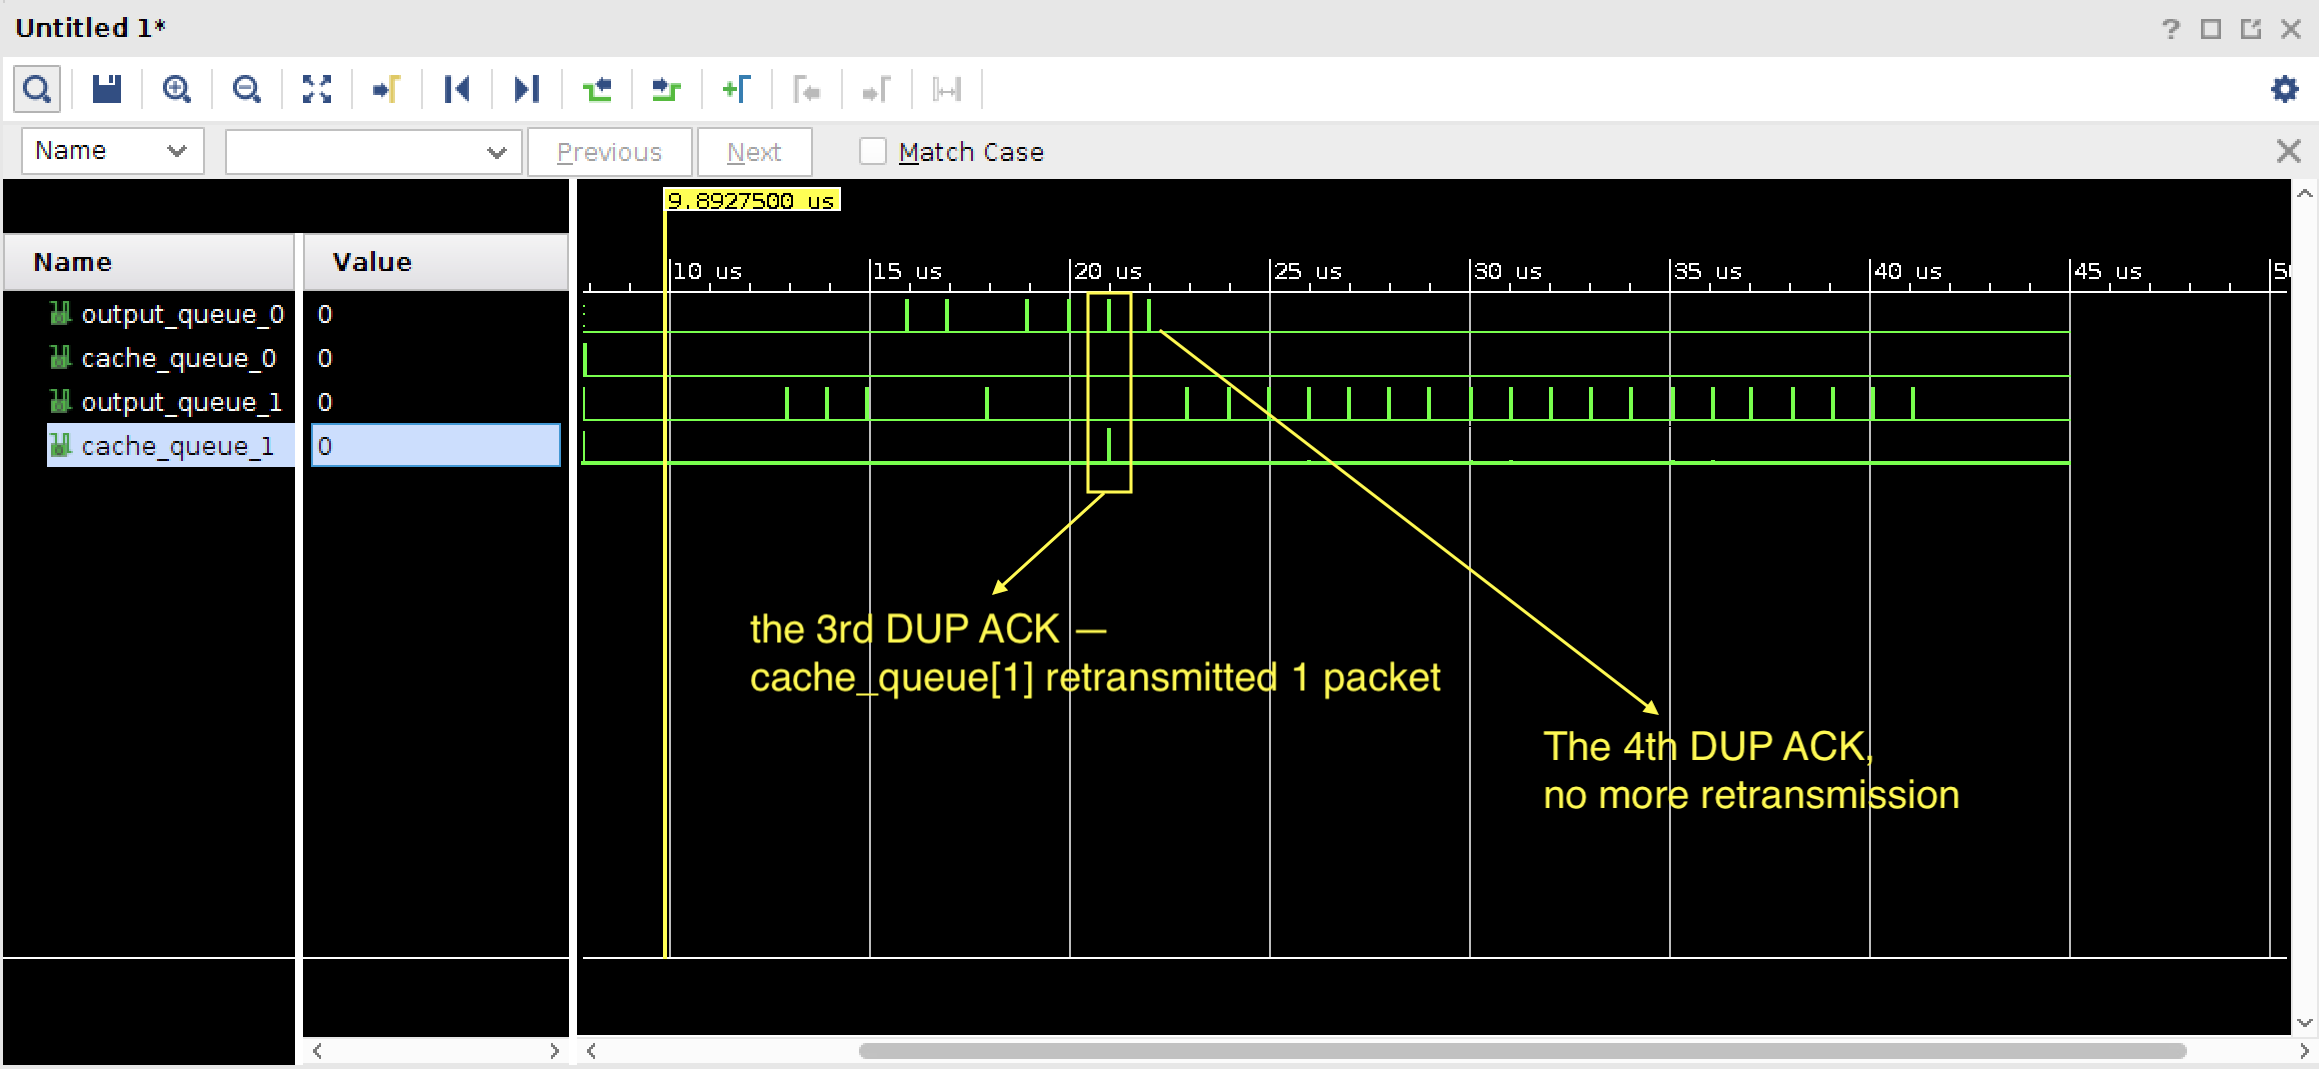
\includegraphics[width=\textwidth]{sume-sim.png}
	\caption{Snapshot of Vivado Design Suite GUI showing the traces of the packets coming out of port \texttt{nf0} and \texttt{nf1} of both the output queue and the cache queue. There is a retransmission on the third DUP ACK packet, but none on the fourth.}
	\label{fig:sumesim}
\end{figure}

\section{Hardware Test}
\label{sec:hwtest}
After all simulations indicated that the P4 implementation is working correctly, I built the FPGA bitstream and tested the functionality of my design on the NetFPGA SUME board. The NetFPGA platform enables running the same tests as in simulations on hardware, with the exception of the limited number of NIC ports (2). Since the number of NIC ports does not affect my design's behaviour, I decided to use the same tests from the SUME simulation. 

The setup for the hardware test requires a machine with the NetFPGA SUME board and a 10Gb NIC, connected as shown in Figure \ref{fig:hwsetup}. The switch passed the hardware tests, as shown by the test output log in Figure \ref{fig:hwlog}, indicating that the switch is fully functional.

\begin{figure}[!h]
	\begin{minipage}{.48\textwidth}
		\centering
		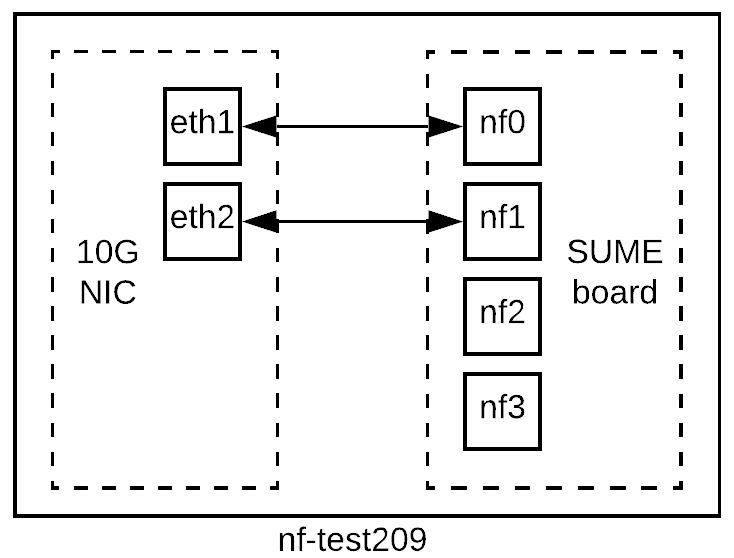
\includegraphics[width=\textwidth]{hwsetup.png}
		\caption{The setup for the hardware test.}
		\label{fig:hwsetup}
	\end{minipage}
	\hfill
	\begin{minipage}{.48\textwidth}
		\centering
		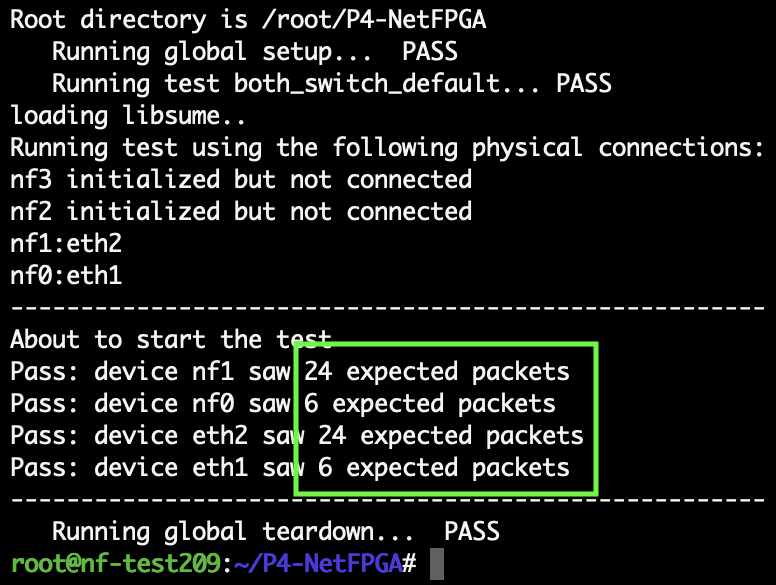
\includegraphics[width=\textwidth]{hwlog.png}
		\caption{Successful test output of the hardware test.}
		\label{fig:hwlog}
	\end{minipage}
\end{figure}

\section{Performance Evaluation}
\label{sec:eval}

\subsection{Performance Analysis}
\label{sec:perf}
I used three metrics to evaluate the performance of the switch: latency, throughput and resources used. The latency and throughput were measured \textit{by my supervisor} on a dedicated setup in the Computer Laboratory data center, to which I have limited access. The setup, as shown in Figure \ref{fig:osnt}, includes one machine with my design programmed onto the SUME board connecting to a second machine with a SUME board that has Open Source Network Tester \cite{osntpdf, osnt} (OSNT) installed on it. OSNT is a fully open-source traffic generator and capture system that is compatible with the NetFPGA-SUME platform. The same setup is also used for unified performance evaluation of other projects, including all Part III P51 course\footnote{\url{https://www.cl.cam.ac.uk/teaching/1819/P51/}} projects.

\subsubsection{Latency}
The latency of the switch was measured by sending 1000 packets of various sizes, ranging from 60B to 1514B, and measuring the round-trip time (RTT) of each packet. The values are then adjusted to compensate for the latency of the setup. The similar experiment was performed on a standard reference switch, and the two results are shown in Figure \ref{fig:latency1}, which plots the average latency against packet size.

As we would expect from a P4 store and forward switch, the latency increases with increasing packet size, ranging from $3250 ns$ to $5340 ns$. In comparison, my device takes $~2500 ns$ longer than the standard switch (i.e. without the cache queue) written in Verilog. This is reasonable since we would expect the retransmit logic to add some overhead to the packet processing time.

\begin{figure}[!h]
	\begin{minipage}{.48\textwidth}
		\centering
		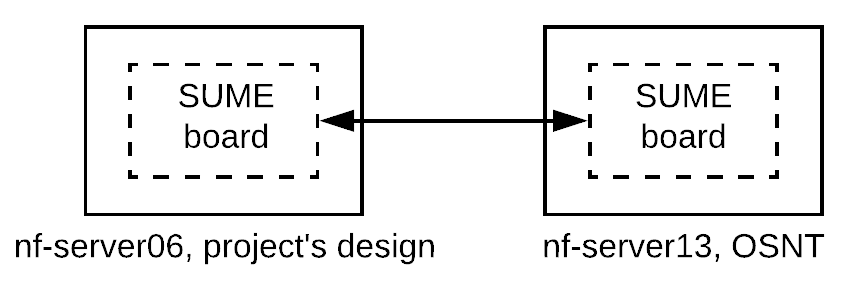
\includegraphics[width=\textwidth]{osnt.png}
		\caption{Setup to measure the latency and throughput of the switch.}
		\label{fig:osnt}
	\end{minipage}
	\hfill
	\begin{minipage}{.48\textwidth}
		\centering
		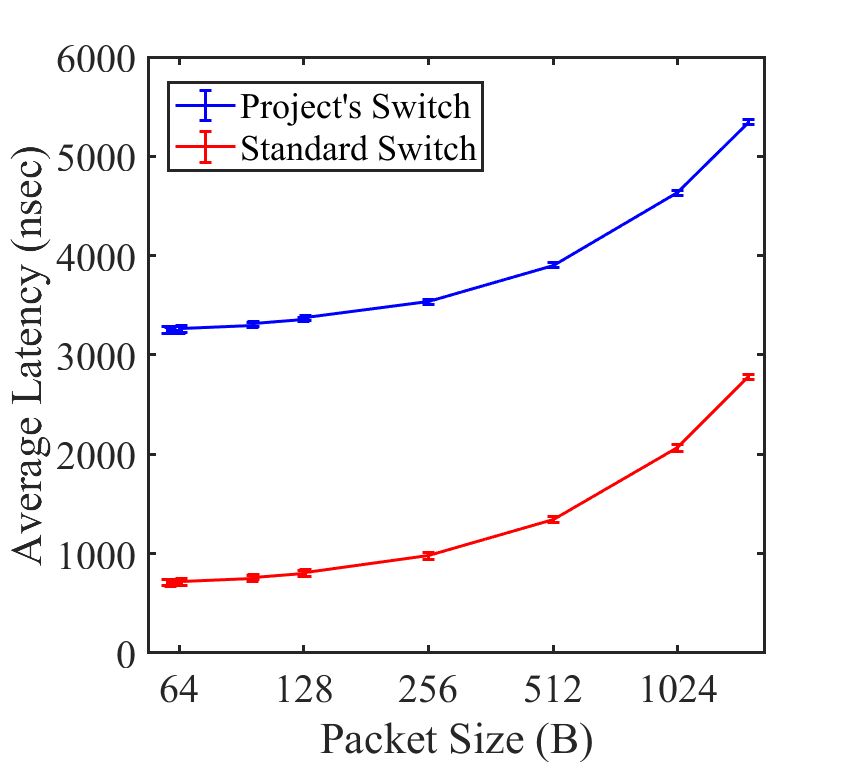
\includegraphics[width=\textwidth]{latency1.png}
		\caption{The average latency of the project's device in comparison with the standard switch. Both are measured by sending 1000 packets of various sizes.}
		\label{fig:latency1}
	\end{minipage}
\end{figure}

\subsubsection{Throughput}
The throughput of the switch was measured on 1 port (Figure \ref{fig:oneport}) and 4 ports (Figure \ref{fig:fourport}) running at the full speed of \textbf{10Gbps/port} (\textbf{40Gbps per design}). In the first case, using 64-Byte packets, packet drops occurred when 100 million packets were sent, while that for 65-Byte packets is 1 billion. Similar results were achieved in the latter case, where packet losses occurred only when 1 billion packets were sent to each of the 4 ports.

As demonstrated in Figure \ref{fig:throughput}, my device achieved $99.9999\%$ throughput most of the time. No confidence interval was given because the error is negligible (3 packets out of 1 billion) and the test was performed once. Ideally, no packet loss is desirable. Nevertheless, the results are reasonable and expected, taking into account subtle clock differences between OSNT and the device under test.

\begin{figure}[h]
	\centering
	\begin{subfigure}[t]{0.45\textwidth}
		\begin{tabular}{|c|c|c|}
			\hline
			Pkt. size            & \multicolumn{1}{c|}{Pkts. sent} & \multicolumn{1}{c|}{Pkts. dropped} \\ \hline
			\multirow{3}{*}{64B} & 10 M.                             & 0                                  \\ \cline{2-3} 
			& 100 M.                            & 15                                 \\ \cline{2-3} 
			& 1 B.                              & 3                                  \\ \hline
			\multirow{3}{*}{65B} & 10 M.                             & 0                                  \\ \cline{2-3} 
			& 100 M.                            & 0                                  \\ \cline{2-3} 
			& 1 B.                              & 3                                  \\ \hline
		\end{tabular}
		\caption{Throughput test on 1 port, using packet size of 64B and 65B.}
		\label{fig:oneport}
	\end{subfigure}
	\hfill
	\begin{subfigure}[t]{0.45\textwidth}
		\begin{tabular}{|c|c|c|}
			\hline
			Pkt. size            & \multicolumn{1}{c|}{Pkts. sent} & \multicolumn{1}{c|}{Pkts. dropped} \\ \hline
			\multirow{3}{*}{64B} & 10 M.                             & 0                                  \\ \cline{2-3} 
			& 100 M.                            & 0                                  \\ \cline{2-3} 
			& 1 B.                              & 1767                               \\ \hline
		\end{tabular}
		\caption{Throughput test on 4 ports, using packet size of 64B.}
		\label{fig:fourport}
	\end{subfigure}
	\caption{Throughput of the switch testing with 1 port \textbf{(a)} and 4 ports \textbf{(b)} running at full speed of 10 Gbps/port. B: Bytes, M.: Million, B.: Billion.}
	\label{fig:throughput}
\end{figure}

\subsubsection{Resources Used}
When we compiled the NetFPGA bitstream, Vivado synthesised and implemented the design, and provided us with a summary of the timing analysis and resources usage. Figure \ref{fig:tsa} shows that our implementation \textit{passed} the timing analysis---all the timing constraints we imposed are satisfied. Figure \ref{fig:memory} shows the utilisation statistics of two of the resources---the memory and the LUTs---of both devices. We can see that our device used more resources than the reference switch: more than $30\%$ LUTs and $60\%$ memory. This is likely due to the larger number of computations and registers used by our P4 program. 

\begin{figure}[!h]
	\centering
	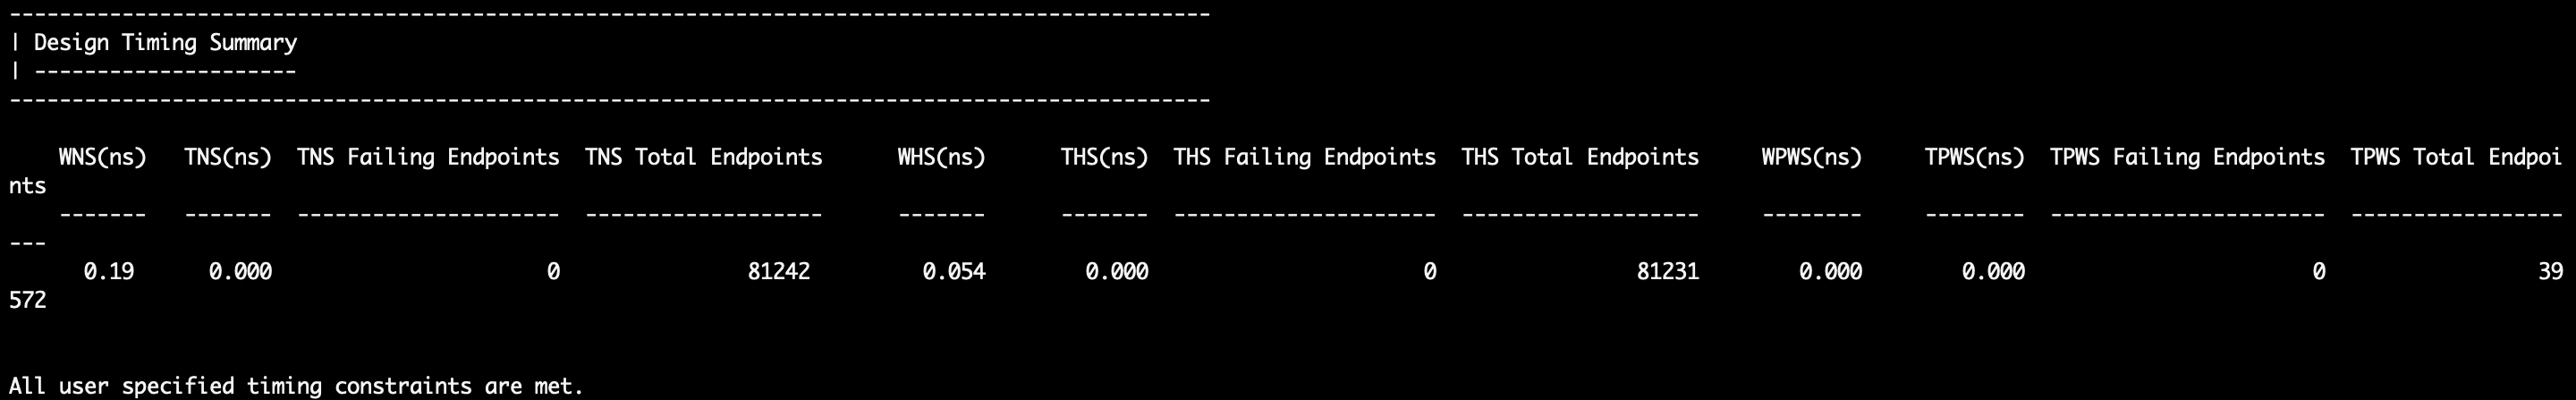
\includegraphics[width=\textwidth]{tsa.png}
	\caption{An extract from the Timing Analysis Report of Vivado showing our design met all the timing constraints.}
	\label{fig:tsa}
\end{figure}

\begin{figure}[h]
	\centering
	\begin{subfigure}[b]{0.45\textwidth}
		\centering
		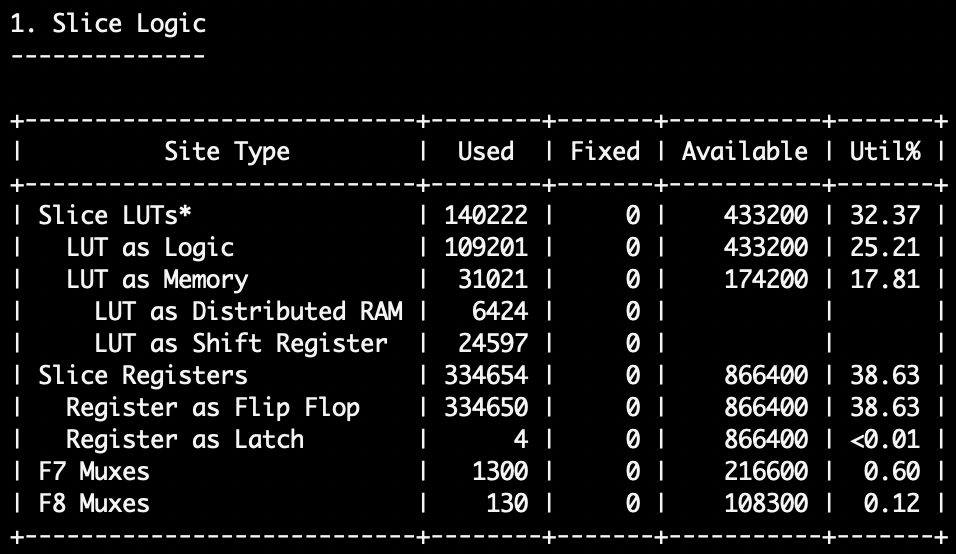
\includegraphics[width=\textwidth]{lut.png}
		\caption{Slice logic utilisation of project device.}
	\end{subfigure}
	\hfill
	\begin{subfigure}[b]{0.45\textwidth}
		\centering
		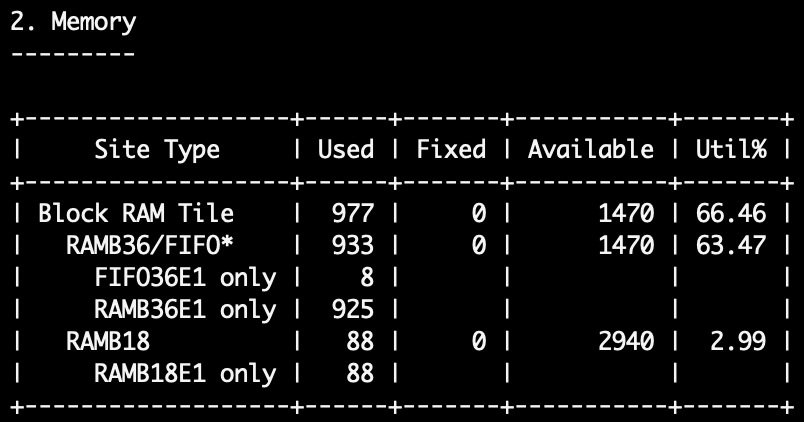
\includegraphics[width=\textwidth]{memory.png}
		\caption{Memory utilisation of project device.}
	\end{subfigure}
	\begin{subfigure}[b]{0.45\textwidth}
		\centering
		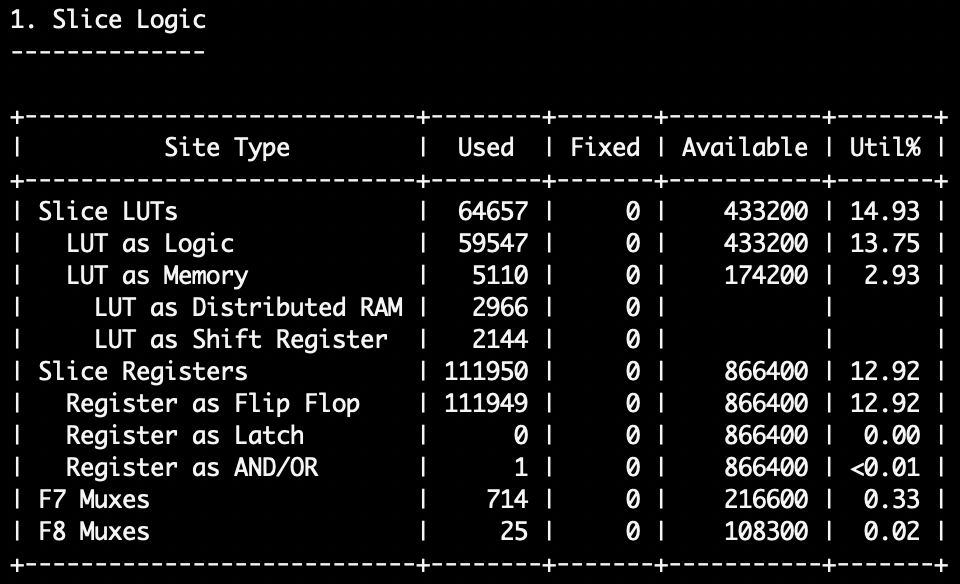
\includegraphics[width=\textwidth]{lut1.png}
		\caption{Slice logic utilisation of reference switch.}
	\end{subfigure}
	\hfill
	\begin{subfigure}[b]{0.45\textwidth}
		\centering
		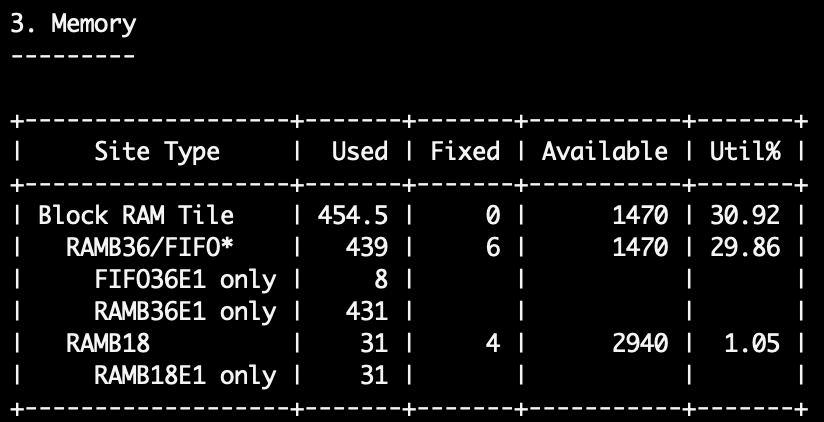
\includegraphics[width=\textwidth]{memory1.png}
		\caption{Memory utilisation of reference switch.}
	\end{subfigure}
	\caption{Specialised resources usage extracted from the device utilisation statistics report of Vivado.}
	\label{fig:memory}
\end{figure}

\subsection{Interoperability}
\label{sec:interop}
To demonstrate the interoperability of the device, we connect it between the two 10Gb NIC of two machines, as shown in Figure \ref{fig:interop}. Then, we run some simple applications between the two machines and observe if the switch is able to deliver the packets. In this project, I demonstrated using \verb|ping| and \verb|iperf3|. In the first setup, we ping from \verb|10.0.0.1| to \verb|10.0.0.2| and capture the packets on \verb|10.0.0.2| with \verb|tcpdump| for visualisation. In the second setup, we run \verb|iperf3| server on \verb|10.0.0.2| and client on \verb|10.0.0.1|. The outputs of both setups are shown in Figure \ref{fig:tcpdump} and \ref{fig:iperf} respectively, indicating the interoperability of the device. I should note that the numbers in Figure \ref{fig:iperf} may well be an underestimate of my device's capability. This could be due to \verb|iperf3| trying to send packets of size larger than 64B, while my device only handles a single packet size of 64B.

\begin{figure}[!h]
	\centering
	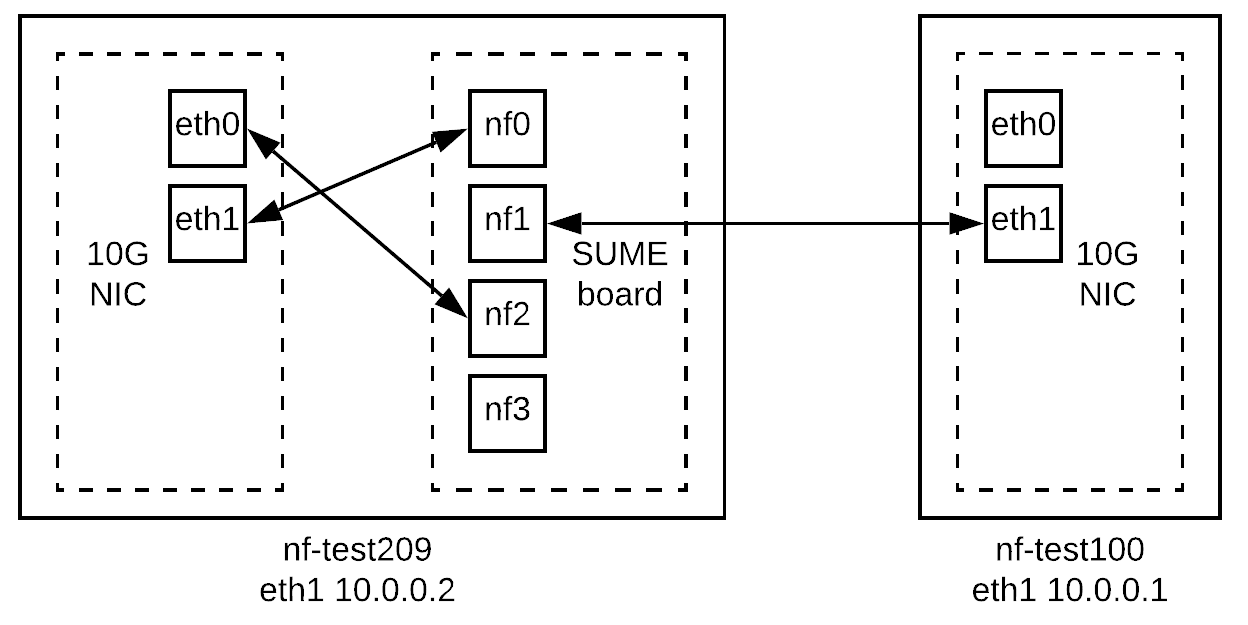
\includegraphics[width=0.7\textwidth]{interop.png}
	\caption{Setup to demonstrate the interoperability of the switch.}
	\label{fig:interop}
\end{figure}

\begin{figure}[!h]
	\centering
	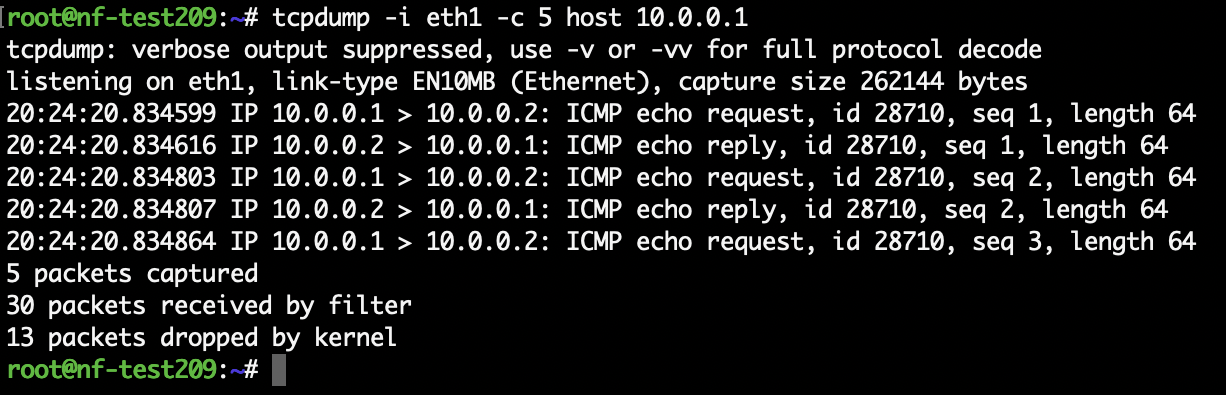
\includegraphics[width=\textwidth]{tcpdump.png}
	\caption{Output of running \texttt{tcpdump} on \texttt{10.0.0.2} capturing packets to and from \texttt{10.0.0.1}.}
	\label{fig:tcpdump}
\end{figure}

\begin{figure}[!h]
	\centering
	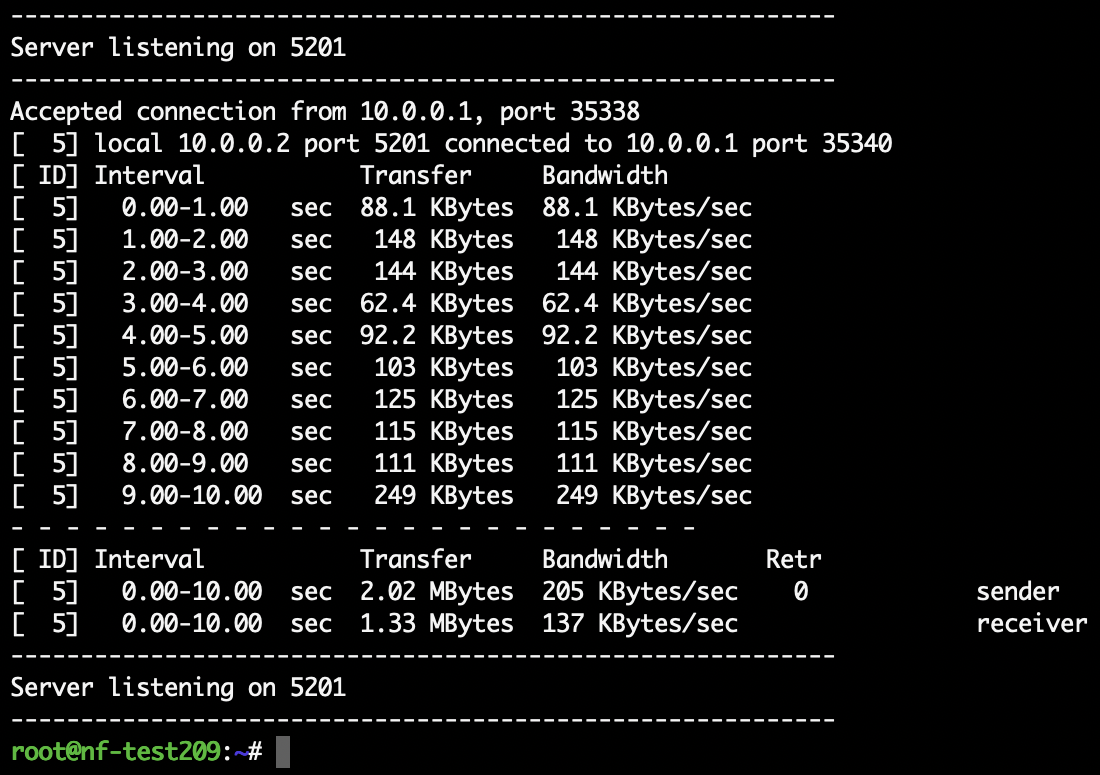
\includegraphics[width=0.8\textwidth]{iperf.png}
	\caption{Output from the \texttt{iperf3} server machine.}
	\label{fig:iperf}
\end{figure}

\subsection{Limitations}
\label{sec:limit}
The design has been assessed for correctness (via simulations), functionality (via functional system test), performance and interoperabilty. While the results have been positive, I have not been able to demonstrate the performance improvement of the switch under an interoperability scenario. In other words, I have also attempted to measure the time in performing real tasks such as file transferring (using \verb|scp|) with and without my design, but there is no signifcant difference in the performance.
